\begin{multicols}{2}
\section*{Objetivo General}
\normalsize{Determinar experimentalmente la aceleración gravitacional $g$ a partir de un experimento de caída libre.}\\
\section*{Objetivos específicos}
%\normalsize{
\begin{enumerate}
    \item Medir desplazamientos para un objeto en caída libre.
    \item Representar el movimiento del objeto mediante la construcción de gráficos que faciliten su análisis.
    \item Determinar la aceleración gravitacional $g$ experimentalmente.
\end{enumerate} 
%}\\
\section*{Referentes conceptuales}
El movimiento de un cuerpo en caída libre bajo la influencia de la gravedad es un ejemplo de aceleración constante. Esta aceleración, llamada aceleración gravitacional (g), tiene un valor aproximado de 9.77 m/s² en Bogotá, según un reporte de 1997, y está dirigida hacia el centro de la Tierra, ignorando factores como la rotación terrestre y la resistencia del aire.

\begin{center}
    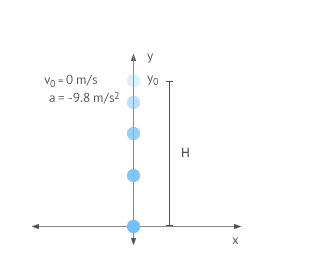
\includegraphics[scale=0.5]{fig/caida-libre.png}
\end{center}

La ecuación (\ref{eq1}) permite obtener la posición de un cuerpo en función del tiempo para una aceleración constante. Si el movimiento es completamente vertical su velocidad aumenta.

\begin{align}\label{eq1}
    y(t) = y_o + v_o \cdot t  - \dfrac{g t^2}{2}
\end{align}

Donde $y(t)$ representa la posición, $g$ la aceleración y $t$ el tiempo. Si el cuerpo “cae” desde el reposo $(v_o = 0)$ en un tiempo inicial $t_o = 0$. Si se define como $y_o = 0$ el punto desde donde se deja caer, por consiguiente, la ecuación anterior se reduce a:

\begin{align} \label{eq2}
    y(t) = - \dfrac{g t^2}{2}
\end{align}

\section*{Actividades Previas}   
\begin{enumerate}
\item Después de observar el vídeo: \\ \href{https://www.youtube.com/watch?v=Y4AJo-Ana70}{https://www.youtube.com/watch?v=Y4AJo-Ana70}. La relación y la diferencia entre las constantes $G$ y $g$ es: ...
\item  En el punto más alto de una caída libre la velocidad siempre es 0 debido a que este es el punto donde se inicia el movimiento, y por ende no se le aplica una velocidad inicial, de lo contrario sería tiro vertical. 
        Sin embargo la aceleración es constante y su valor es de $-9.8 m/s^2$.
\item Diferencias y semejanzas que pueda tener un objeto en caída libre y un objeto lanzado de forma vertical hacia arriba:\\
    \textbf{Diferencias:}
    \begin{itemize}
        \item Un objeto en caída libre se mueve únicamente bajo la influencia de la gravedad, mientras que un objeto lanzado verticalmente hacia arriba tiene una velocidad inicial en contra de la gravedad.
    \end{itemize}

    \textbf{Semejanzas:}
    \begin{itemize}
        \item Los objetos en ambos movimientos tienen una aceleración constante en la dirección de la gravedad.
        \item Los objetos en ambos movimientos tienen una velocidad inicial o final de 0 (dependiendo si es caída libre o tiro vertical respectivamente) en el punto más alto de su trayectoria.
        \item Al alcanzar el punto más alto en un tiro vertical, el movimiento se transforma en caída libre.
    \end{itemize}
\item Tres personas fueron importantes para hallar la aceleración gravitacional:\\
    \textbf{Galileo Galilei:} Realizó experimentos con planos inclinados y péndulos, y demostró que la aceleración de la gravedad es constante.\\
    \textbf{Isaac Newton:} Propuso la ley de la gravitación universal, que describe la fuerza de atracción entre dos cuerpos.\\
    \textbf{Henry Cavendish:} El experimento de Cavendish fue diseñado para medir la atracción gravitacional entre objetos pequeños. 
    Usó una balanza de torsión, que consistía en una barra horizontal suspendida por un alambre delgado. En cada extremo de la barra había una esfera de plomo. 
    Cavendish midió la fuerza de atracción entre las dos esferas de plomo \textbf{de diferentes tamaños} y calculó la masa de la Tierra.

    \begin{figure}[H]
        \centering
        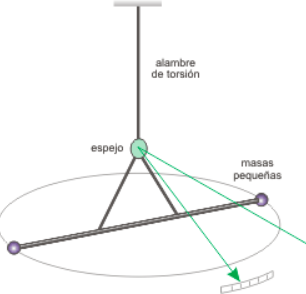
\includegraphics[scale=0.7]{fig/procesoCavendish-gravedad.png}
        \caption{Proceso de Cavendish para medir la gravedad}
    \end{figure}
\end{enumerate}
    
\section*{Materiales de Laboratorio}  
$\cdot$ Un celular con la aplicación PhyPhox establecida en el modo cronómetro acústico\\
$\cdot$ 30 globos\\
$\cdot$ Un flexómetro\\
$\cdot$ Una moneda de \$500\\
    \begin{center}
        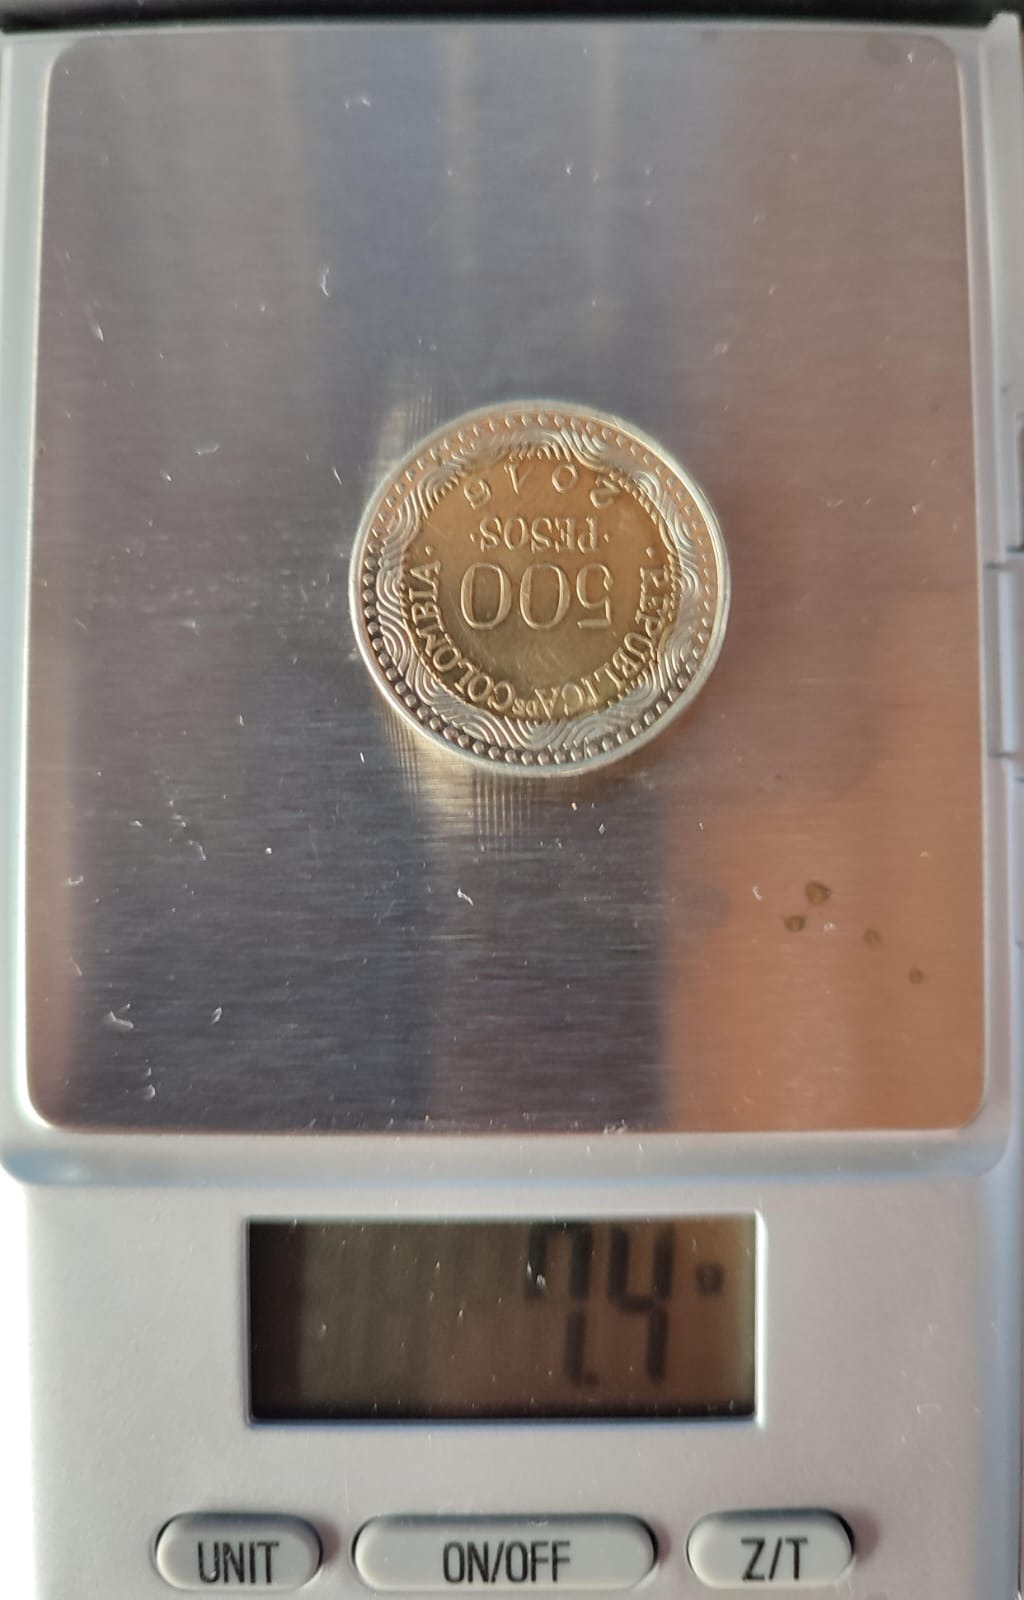
\includegraphics[scale=0.05]{fig/moneda.png}\\
    \end{center}
$\cdot$ Una pieza metálica\\
    \begin{center}
        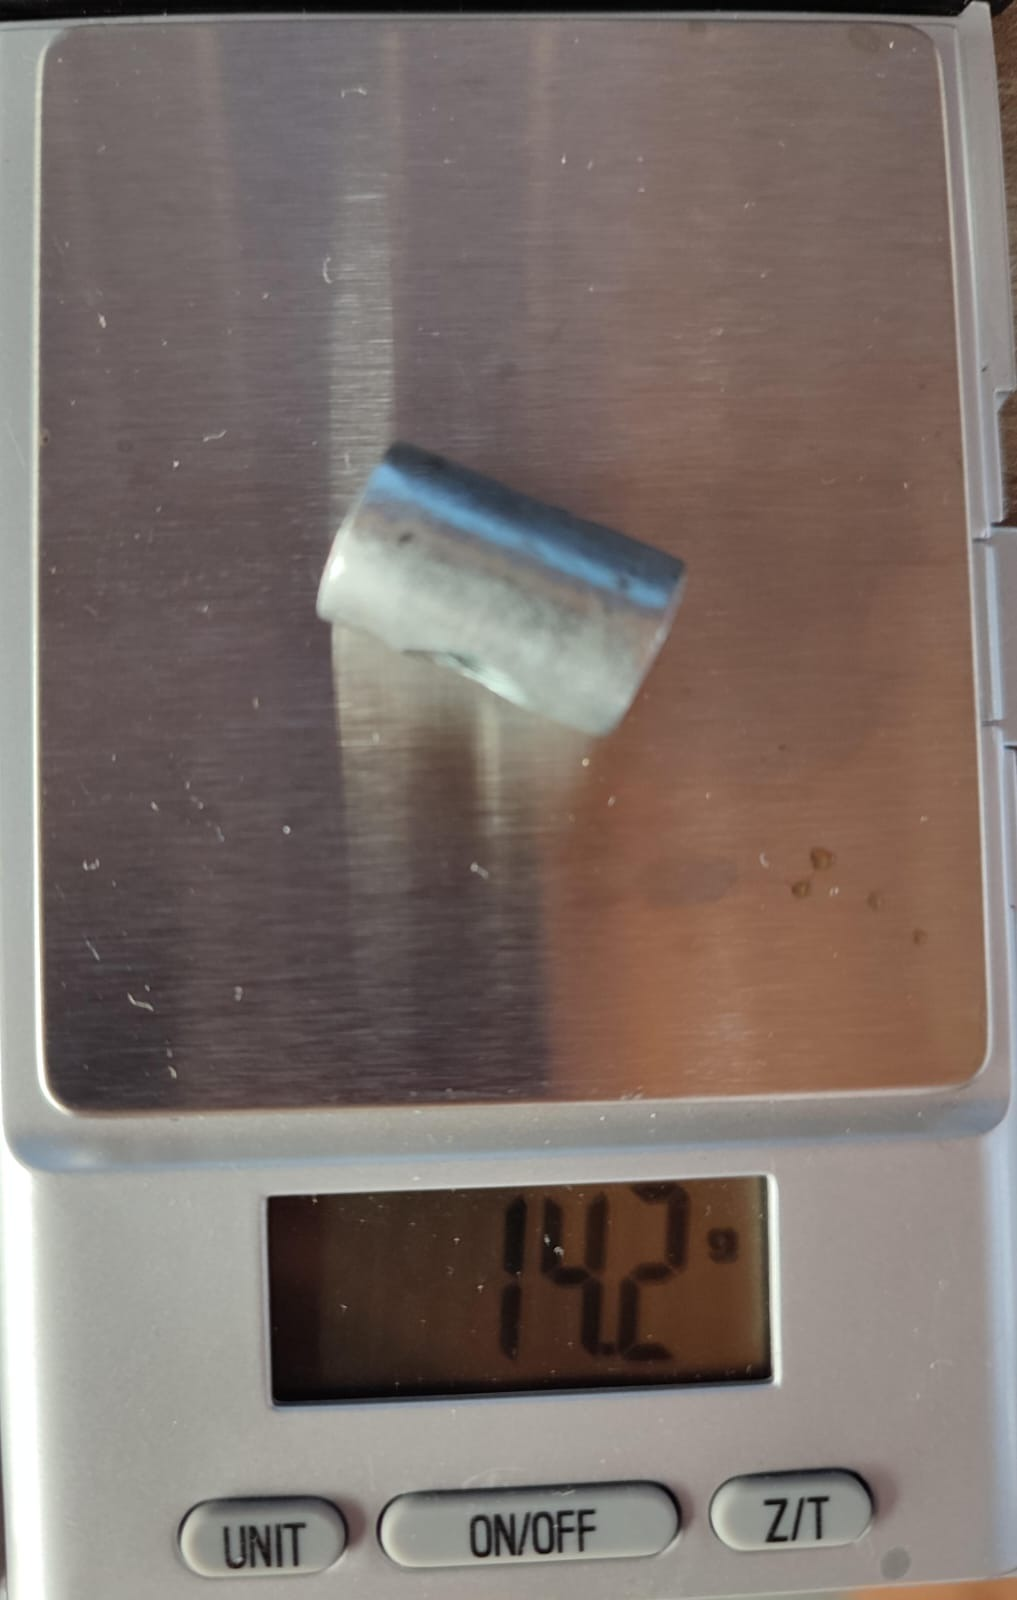
\includegraphics[scale=0.05]{fig/pieza-metalica.png}
    \end{center}

\section*{Procedimiento}
\begin{enumerate}
    \item Ingresar a la aplicación y elegir el cronómetro acústico.

    \item En modo simple, se estableció el valor del “Umbral” a 0.2 y el “Retraso Mínimo” a 0.1
    
    \item Elegir un área que cuente con una altura moderada y en la cual se tenga una superficie que pueda ser impactada, en este laboratorio se eligió la terraza de una casa. 
    
    \item Ubicar el móvil sobre una base sólida de forma que el micrófono no se encuentre obstruido y pueda tener mayor sensibilidad auditiva.
    
    \item Al explotar la bomba, se producirá el sonido que indica el comienzo de la caída del objeto (inicia el cronómetro), inmediatamente el objeto cae.
    
    \item Tomar tres mediciones de tiempo (Medida 1, Medida 2 y Medida 3) para 5 alturas diferentes y registrar los datos en la tabla 1.
    
    \item Cambiar el objeto por uno de mayor o menor peso, repetir los puntos 8 al 9, y registrar los datos en la tabla 2.
\end{enumerate}

\begin{figure}[H]
    \centering
    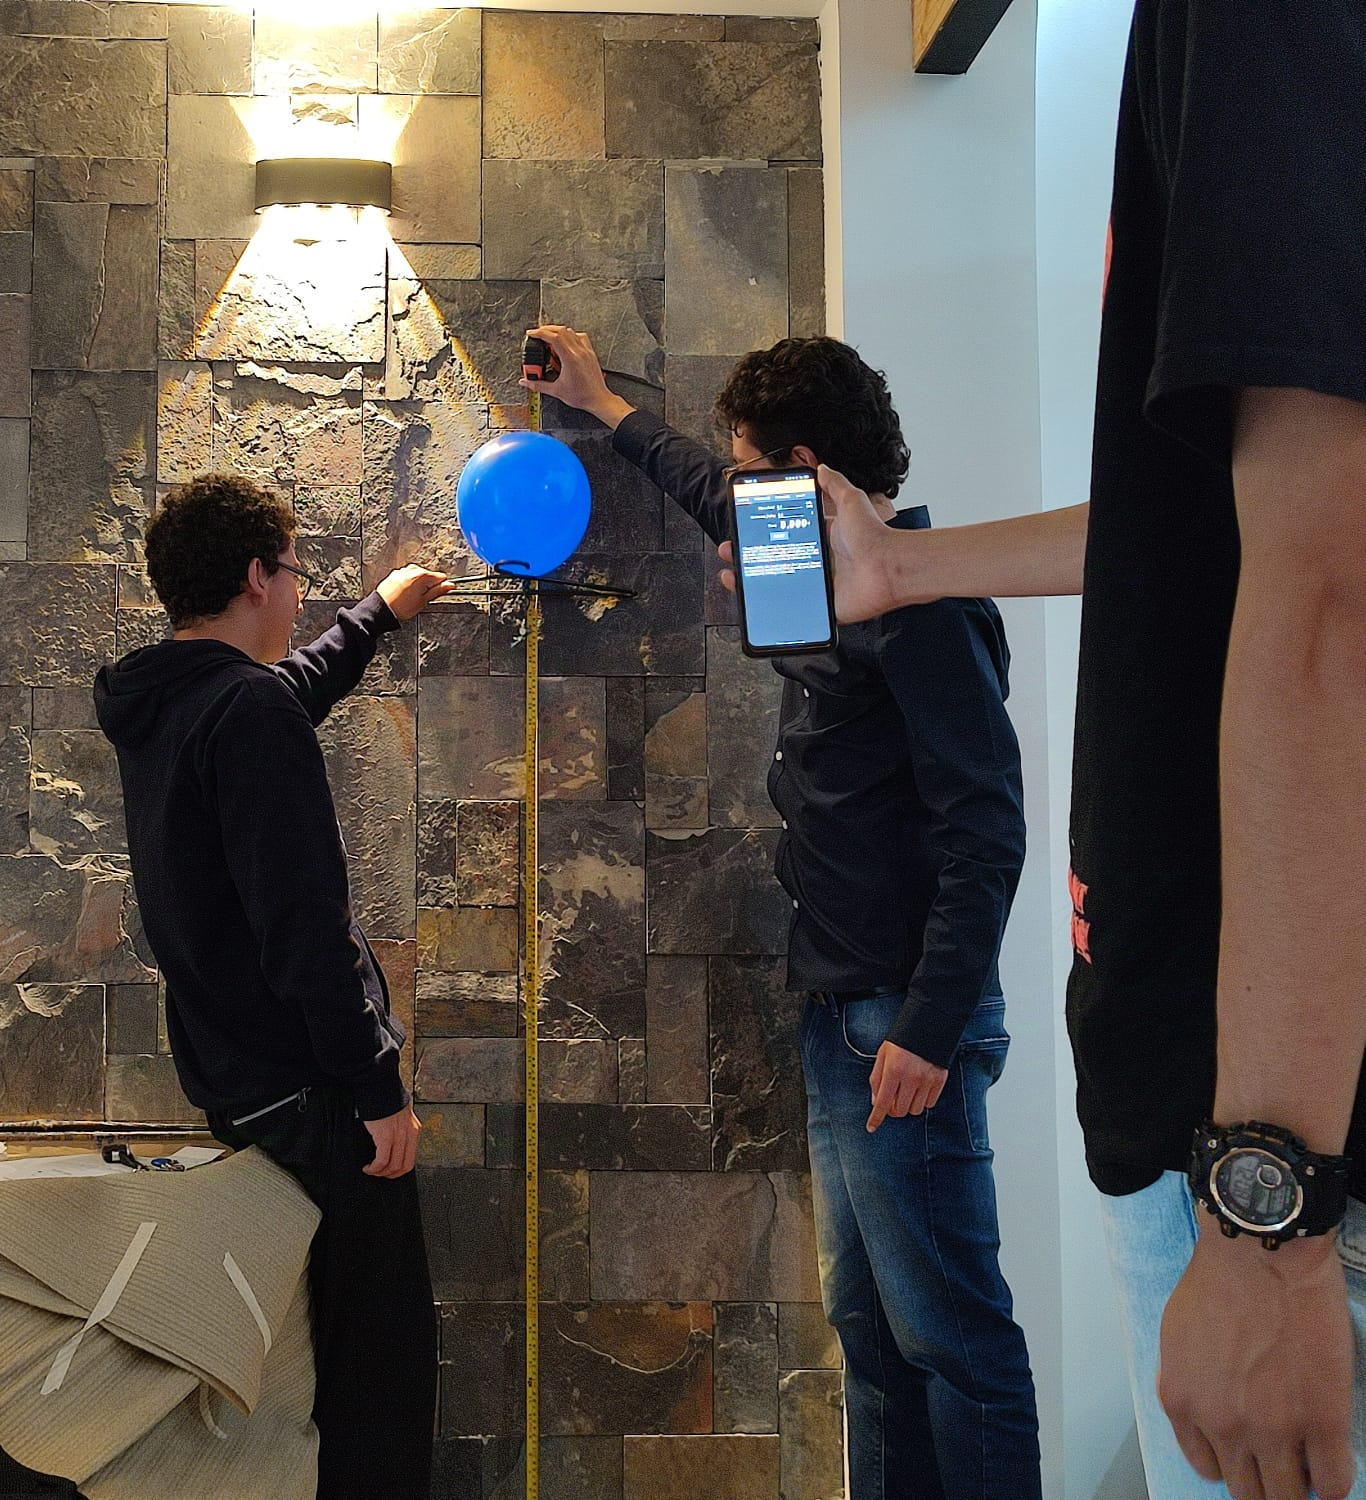
\includegraphics[scale=0.1]{fig/procedimiento.png}
    \caption{Procedimiento}
    \label{fig:procedimiento}
\end{figure}

\section*{Resultados}
%Tabla 1
\begin{figure}[H]
    \centering
    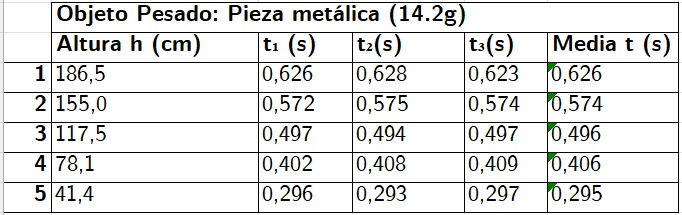
\includegraphics[scale=0.3]{fig/Tabla1-ObjetoPesado.png}
    \caption{...}
    \label{fig:tabla1}
\end{figure}

%Tabla 2
\begin{figure}[H]
    \centering
    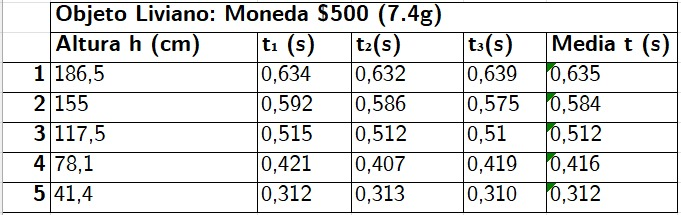
\includegraphics[scale=0.3]{fig/Tabla2-ObjetoLiviano.png}
    \caption{...}
    \label{fig:tabla2}
\end{figure}

\section*{Análisis cuantitativo y cualitativo} 
\textbf{Gráficas}
        \begin{figure}[H]
            \centering
            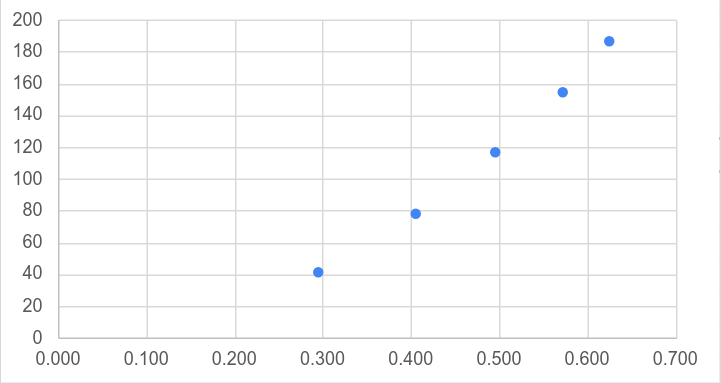
\includegraphics[scale=0.5]{fig/objPesado-Altura-Tiempo.png}
            \caption{Gráfica de Altura vs Tiempo para Objeto Pesado}
        \end{figure}
        
        \begin{figure}[H]
            \centering
            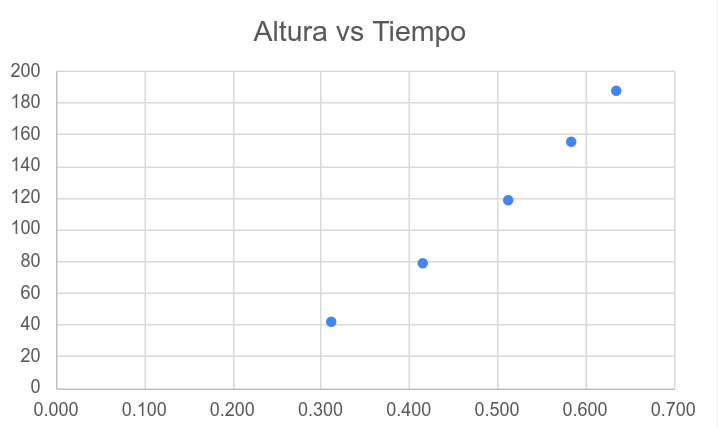
\includegraphics[scale=0.5]{fig/objLiviano-Altura-Tiempo.png}
            \caption{Gráfica de Altura vs Tiempo para Objeto Liviano}
        \end{figure}

\textbf{Regresión por mínimos cuadrados}
%Tabla 3
\begin{figure}[H]
    \centering
    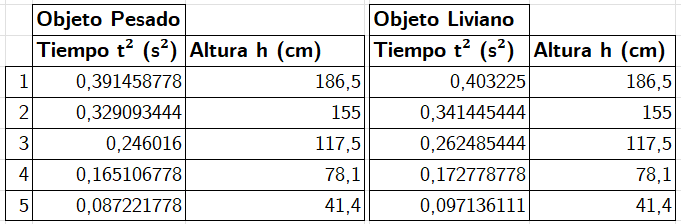
\includegraphics[scale=0.5]{fig/Tabla3-TiempoCuadrado.png}
    \caption[scale=0.5]{Altura vs Tiempo Cuadrado}
\end{figure}

\textit{Nota: } Se decició hacer una regresión polinómica de grado 2 con los datos de las figuras (\ref{fig:tabla1}) y (\ref{fig:tabla2}), teniendo en cuenta los tiempos $t_1$, $t_2$ y $t_3$. De esta manera, se consiguue un valor de la gravedad más preciso.
\begin{figure}[H]
    \centering
    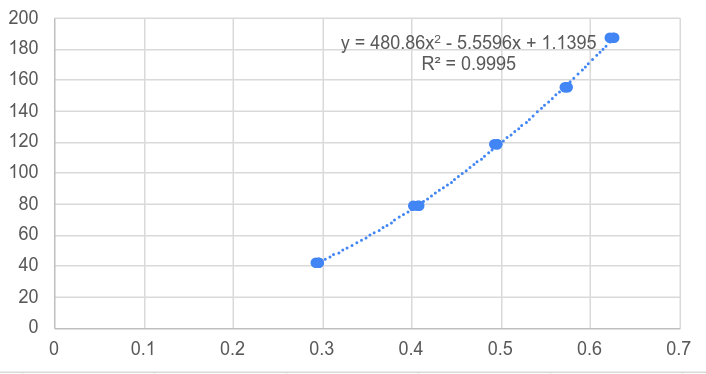
\includegraphics[scale=0.5]{fig/regresion-ObjetoPesado.png}
    \caption{...}
\end{figure}

\begin{figure}[H]
    \centering
    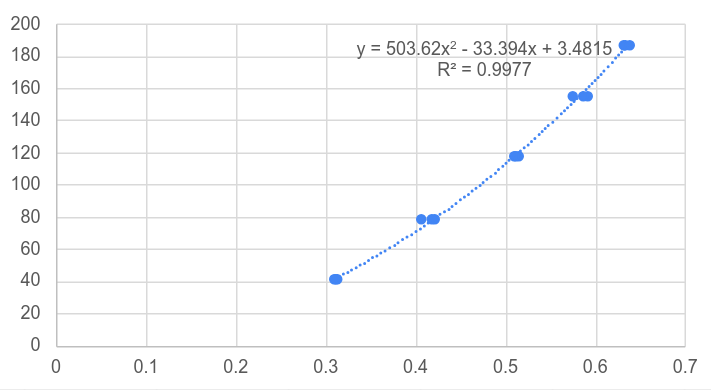
\includegraphics[scale=0.5]{fig/regresion-ObjetoLiviano.png}
    \caption{...}
\end{figure}

\textbf{Determinación de $g$} \\
Se obtuvieron las siguientes ecuaciones:

\begin{align}\label{eq3}
    y = 480.86x^2 - 5.5596x + 1.1395
\end{align}

\begin{align}\label{eq4}
    y = 503.62x^2 - 33.394x + 3.4815
\end{align}

Al usar la ecuación (\ref{eq2}) y compararla con (\ref{eq3}) y (\ref{eq4}), se obtiene que:
\begin{enumerate}
    \item $\dfrac{g}{2} = 480.86 \ cm/s^2$ \hspace{1cm} $g = 9.62 \ m/s^2$
    \item $\dfrac{g}{2} = 503.62 \ cm/s^2$ \hspace{1cm} $g = 10.07 \ m/s^2$
\end{enumerate}

\textbf{Calculo del error porcentual} \\

\[\text{Error\%} = \frac{|g_{\text{teórico}} - g_{\text{experimental}}|}{g_{\text{teórico}}} \times 100 \]

Para el objeto pesado: \[Error = \dfrac{9.77 - 9.62}{9.77} \times 100 = 1.53\%\] \\
Para el objeto liviano: \[Error = \dfrac{9.77 - 10.07}{9.77} \times 100 = 3.07\%\]



\section*{Conclusiones} 
\begin{enumerate}
    \item Cosas a tener en cuenta: ...
    \item Sugerencias para mejorar el experimento: ...
\end{enumerate}
\section*{Referencias bibliográficas}
\small{
$\cdot$ Alonso M. y Finn E. J., “Física” Vol. I, Ed. Addison-Wesley Iberoamericana (1986). \\ 
$\cdot$ Tipler, P.A. Física Vol 1. Ed Reverté, México, (1985).\\
$\cdot$ Sears, F.- Zemansky, M.Física Universitaria I. Ed Pearson, México (1999).\\
$\cdot$ Serway, R. Física I para ciencias e ingeniería. Ed Thomson, México (2005)
}
\end{multicols}